\documentclass[a4paper, 11pt]{article}
\usepackage{graphicx}

\newcommand{\Rfunction}[1]{{\texttt{#1}}}
\newcommand{\Robject}[1]{{\texttt{#1}}}
\newcommand{\Rpackage}[1]{{\textit{#1}}}
\newcommand{\Rmethod}[1]{{\texttt{#1}}}
\newcommand{\Rfunarg}[1]{{\texttt{#1}}}
\newcommand{\Rclass}[1]{{\textit{#1}}}
\newcommand{\Rcode}[1]{{\texttt{#1}}}

\newcommand{\software}[1]{\textsf{#1}}
\newcommand{\R}{\software{R}}
\newcommand{\Bioc}{\software{Bioconductor}}
\newcommand{\IRanges}{\Rpackage{IRanges}}
\newcommand{\biovizBase}{\Rpackage{biovizBase}}
\newcommand{\ggbio}{\Rpackage{ggbio}}
\newcommand{\visnab}{\Rpackage{visnab}}
\newcommand{\ggplot}{\Rpackage{ggplot2}}
\newcommand{\grid}{\Rpackage{grid}}
\newcommand{\gridExtra}{\Rpackage{gridExtra}}
\newcommand{\qplot}{\Rfunction{qplot}}
\newcommand{\biobase}{\software{Bioconductor}}
\newcommand{\nVizN}{\Rpackage{nViZn}}
\begin{document}
\begin{table}[h!t!b!p]
\small{
\begin{tabular}{|p{1cm}|p{2cm}|p{4cm}|p{1cm}|}
\hline
Comp & name  & usage & icon\\\hline
\textbf{geom} &geom\_rect & rectangle& 
\includegraphics[height = 0.5cm]{figure/geom_rect.pdf}\\
              &geom\_segment & segment& 
\includegraphics[height = 0.5cm]{figure/geom_segment.pdf}\\
              &geom\_chevron & chevron&
\includegraphics[height = 0.5cm]{figure/geom_chevron.pdf}\\
              &geom\_arrow & arrow&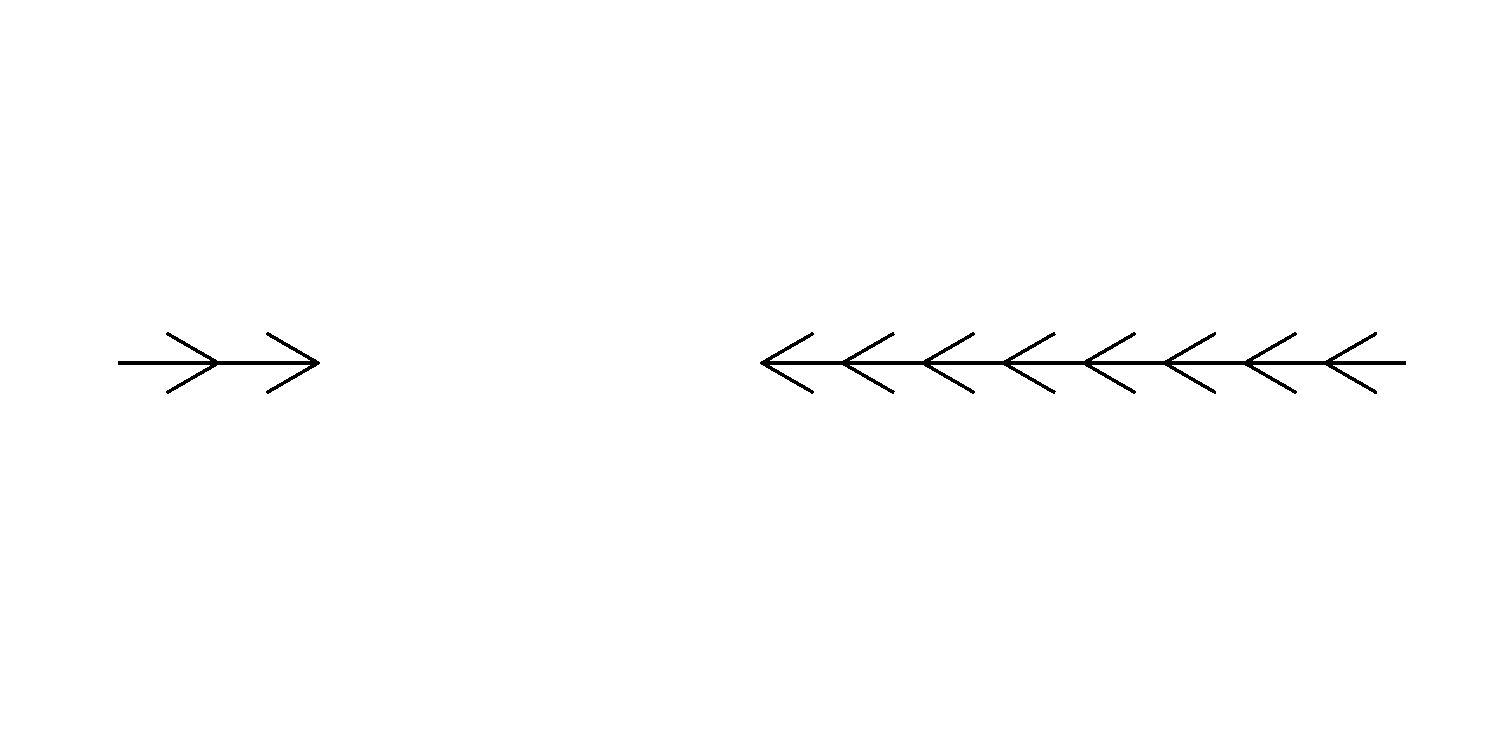
\includegraphics[height = 0.5cm]{figure/geom_arrow.pdf}\\
              &geom\_arch & arches &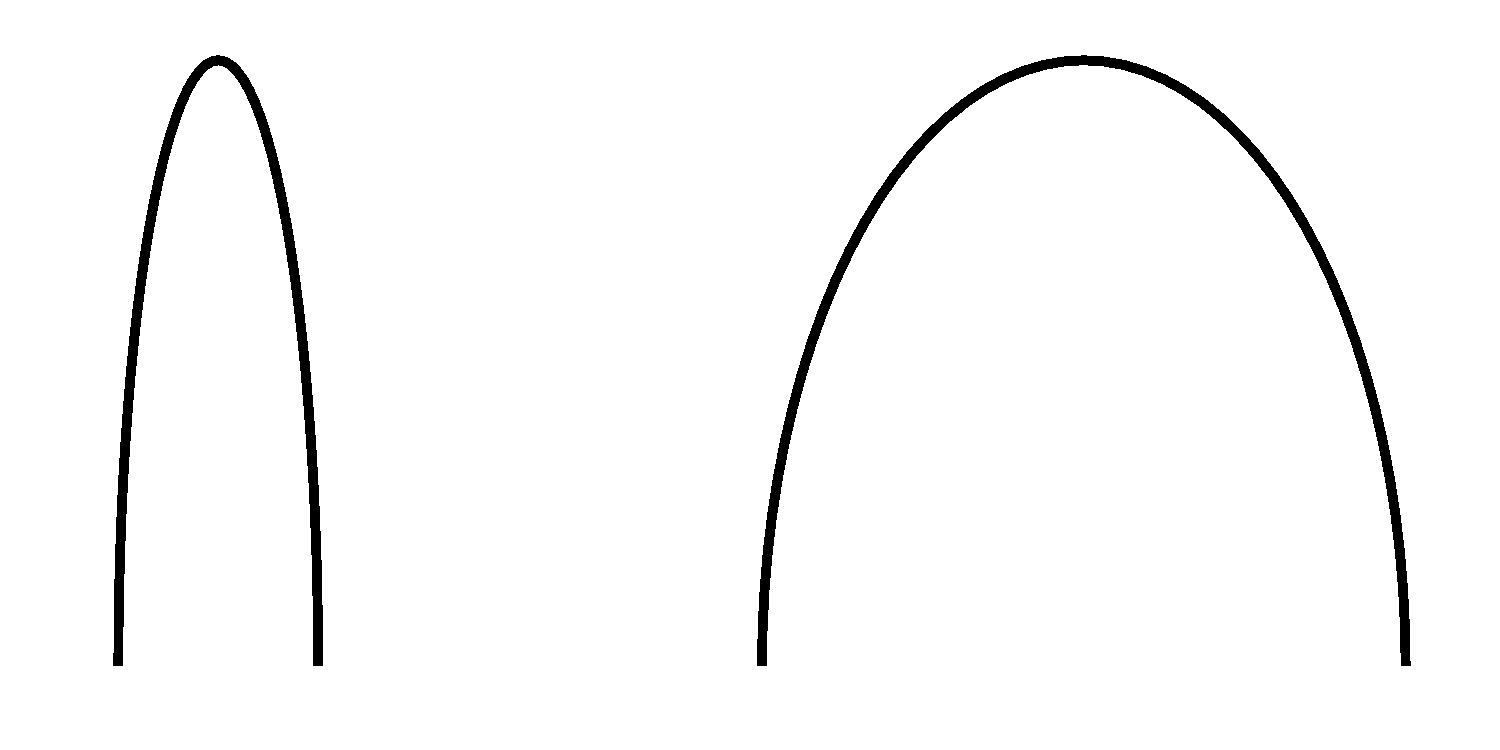
\includegraphics[height = 0.5cm]{figure/geom_arch.pdf}\\
              &geom\_bar & bar &
\includegraphics[height = 0.5cm]{figure/geom_bar.pdf}\\
              &geom\_alignment & gene structure& 
              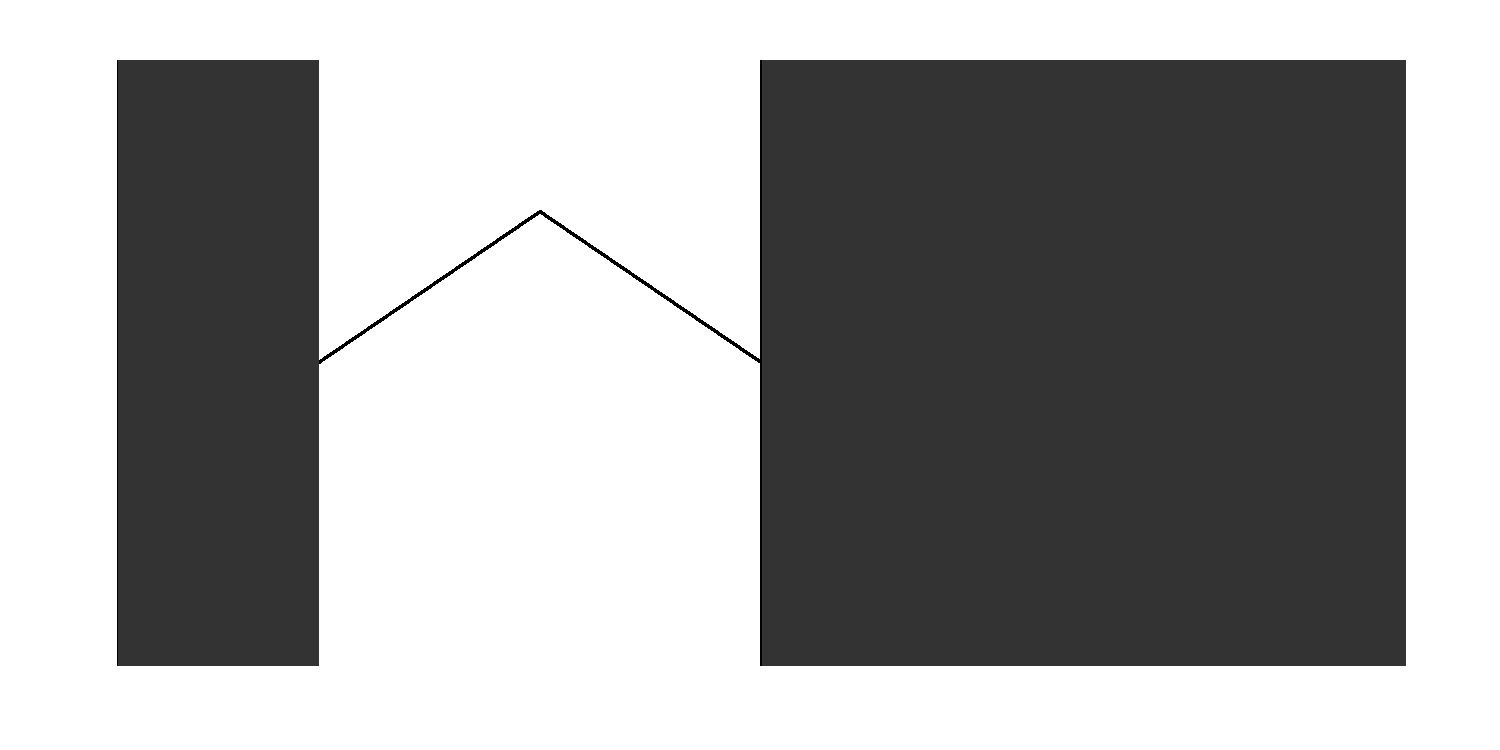
\includegraphics[height = 0.5cm]{figure/geom_alignment.pdf}\\\hline
\textbf{stat} &stat\_aggregate & aggregation in sliding window&
              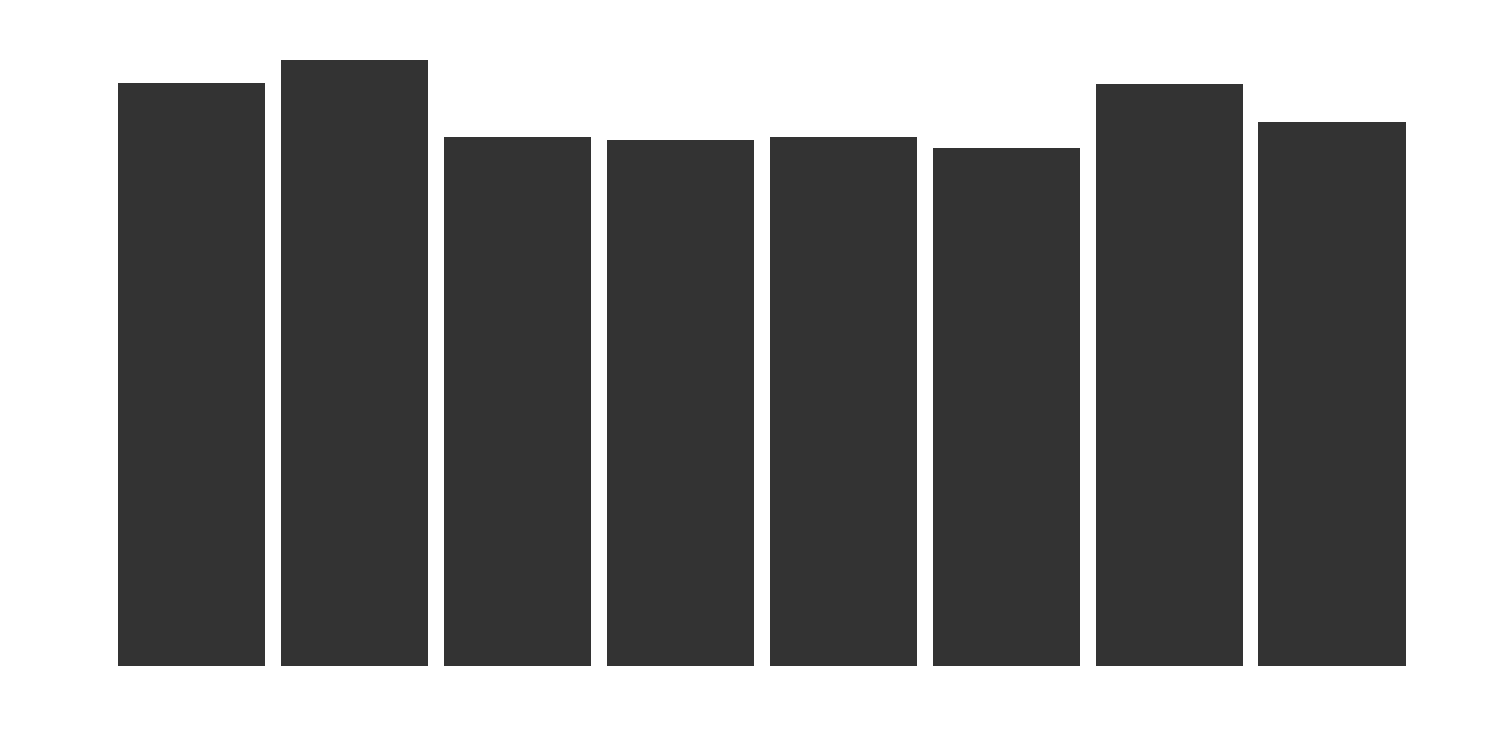
\includegraphics[height = 0.5cm]{figure/stat_aggregate.pdf}\\
              &stat\_coverage & coverage for reads&
              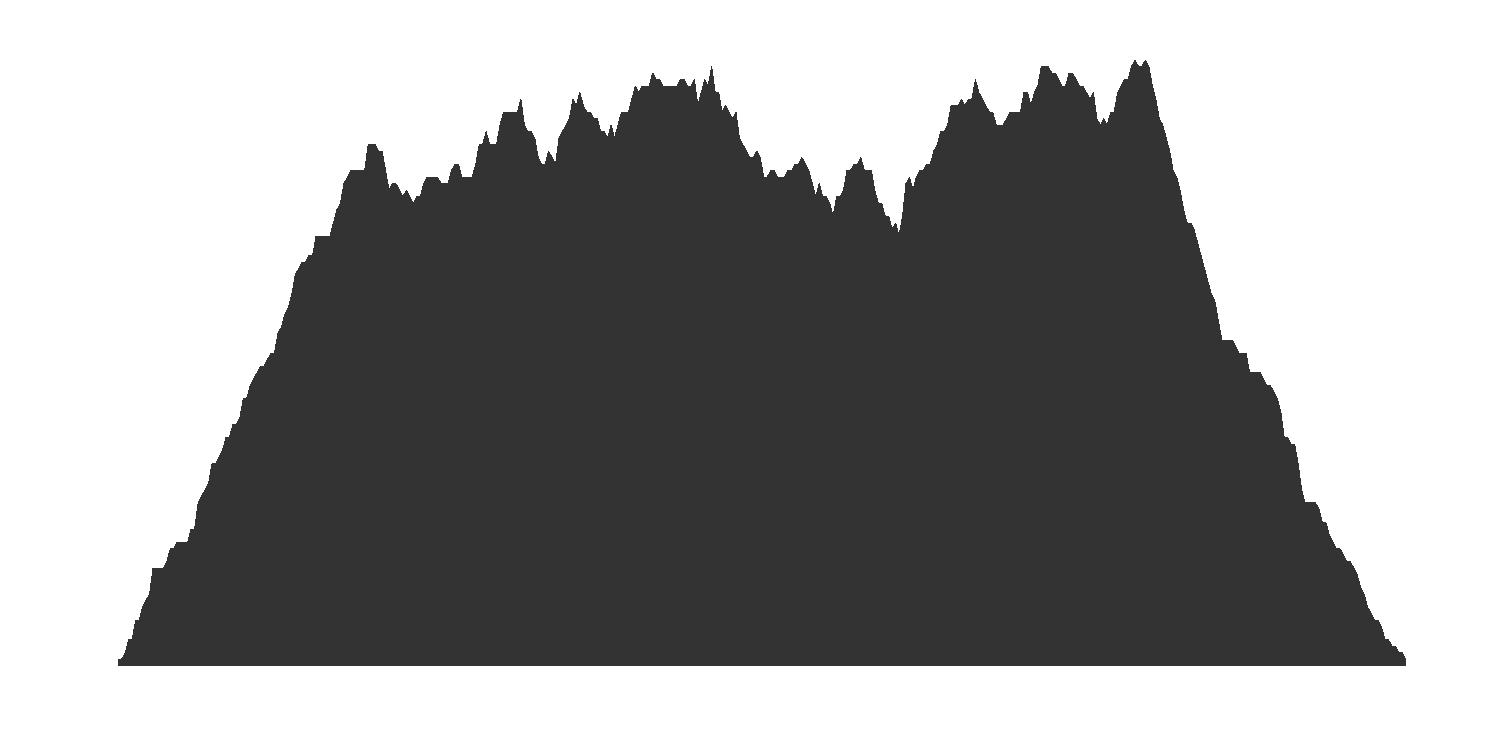
\includegraphics[height = 0.5cm]{figure/stat_coverage_icon.pdf}\\
              &stat\_gene & gene structure&
              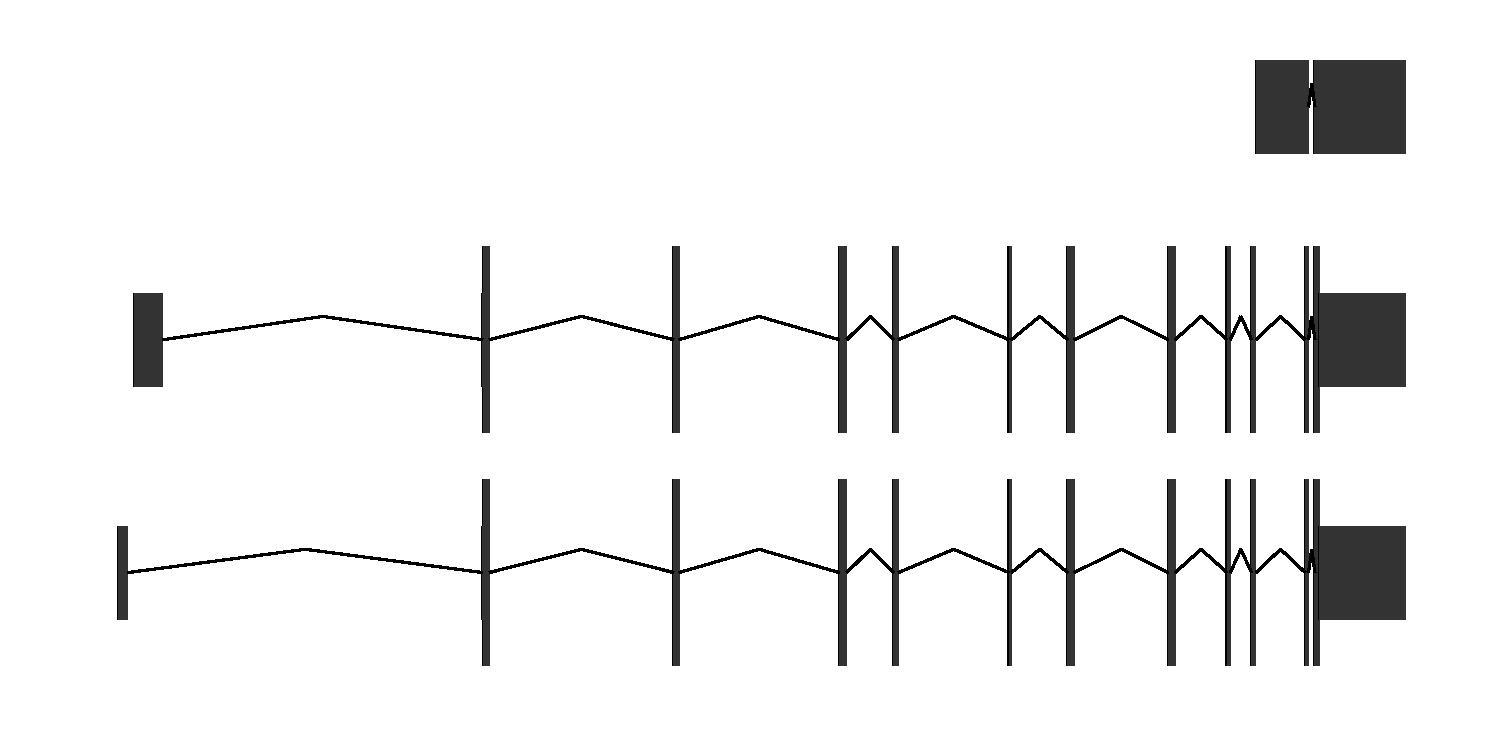
\includegraphics[height = 0.5cm]{figure/stat_gene.pdf}\\
              &stat\_identity & identity mode &
              
\includegraphics[height = 0.5cm]{figure/stat_identity.pdf}\\
              &stat\_mismatch & mismatch summary for variants&
              
\includegraphics[height = 0.5cm]{figure/stat_mismatch.pdf}\\
              &stat\_stepping & stepping levels&
              
\includegraphics[height = 0.5cm]{figure/stat_stepping.pdf}\\
              &stat\_table & tabulate ranges &
              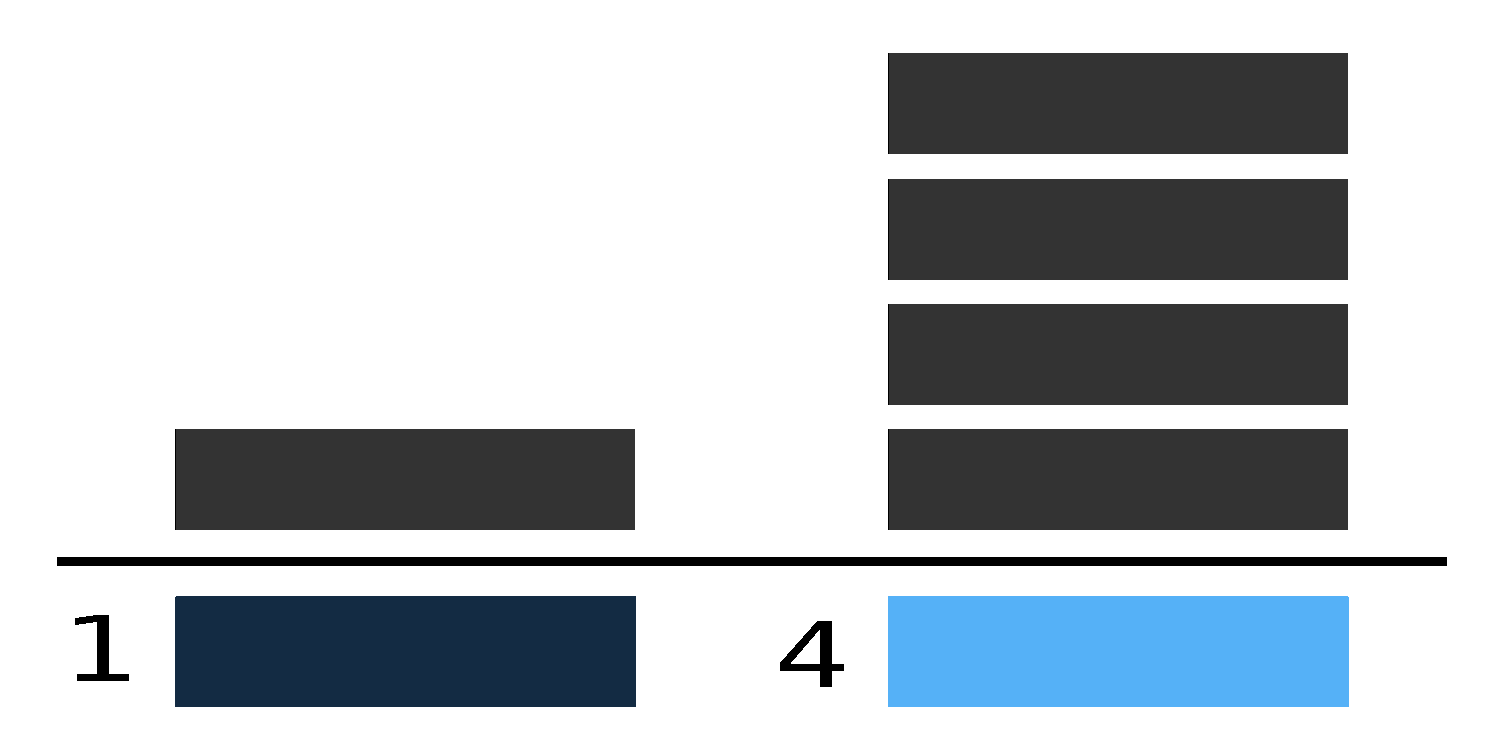
\includegraphics[height = 0.5cm]{figure/stat_table.pdf}\\\hline
\textbf{coord} &linear& default linear but facet by chromosomes space&
               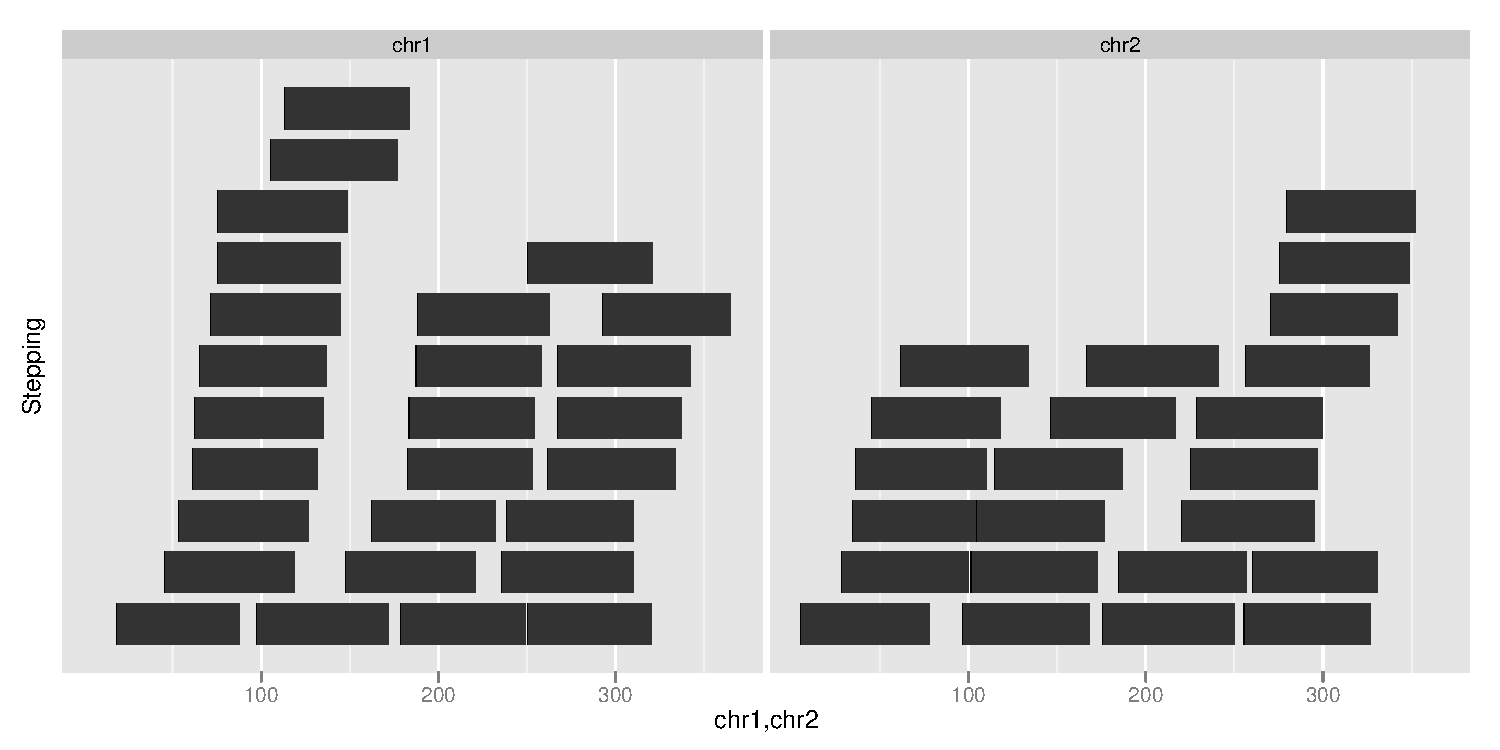
\includegraphics[height = 0.5cm]{figure/coord_linear.pdf}\\
               &genome& put everything on genome coordiante&
               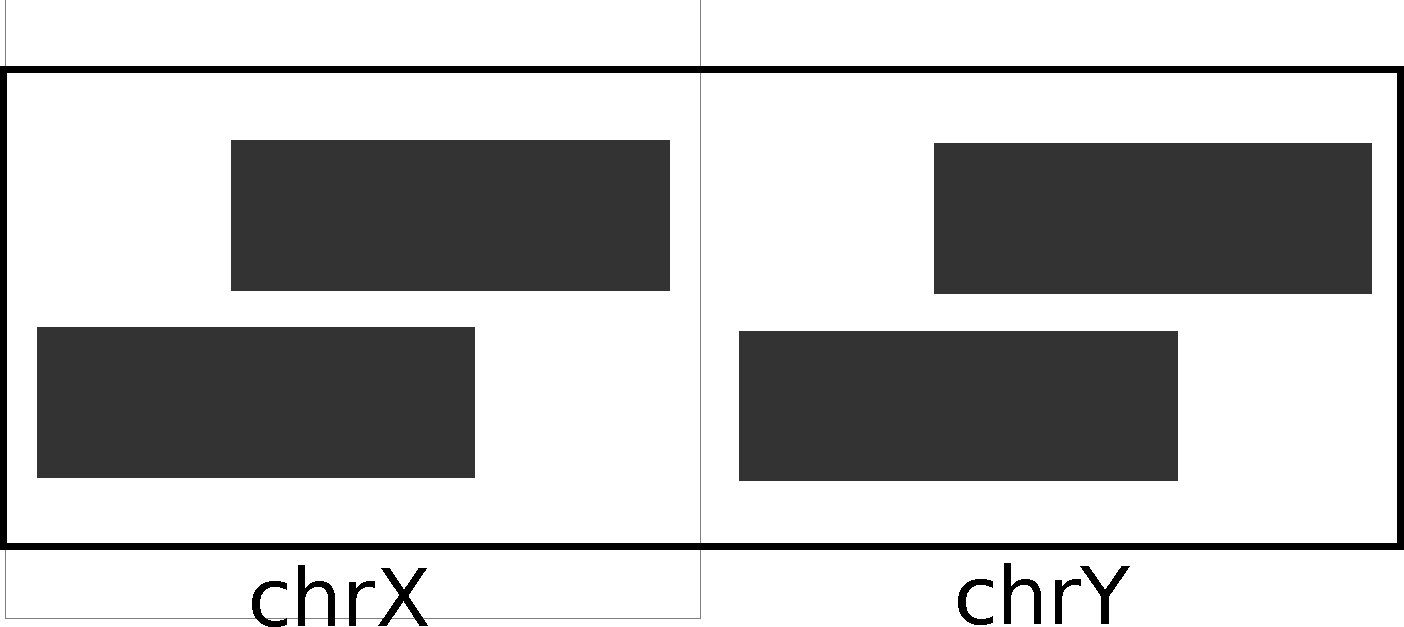
\includegraphics[height = 0.5cm]{figure/coord_genome.pdf}\\
               &truncate gaps & compact view by cutting gaps&
               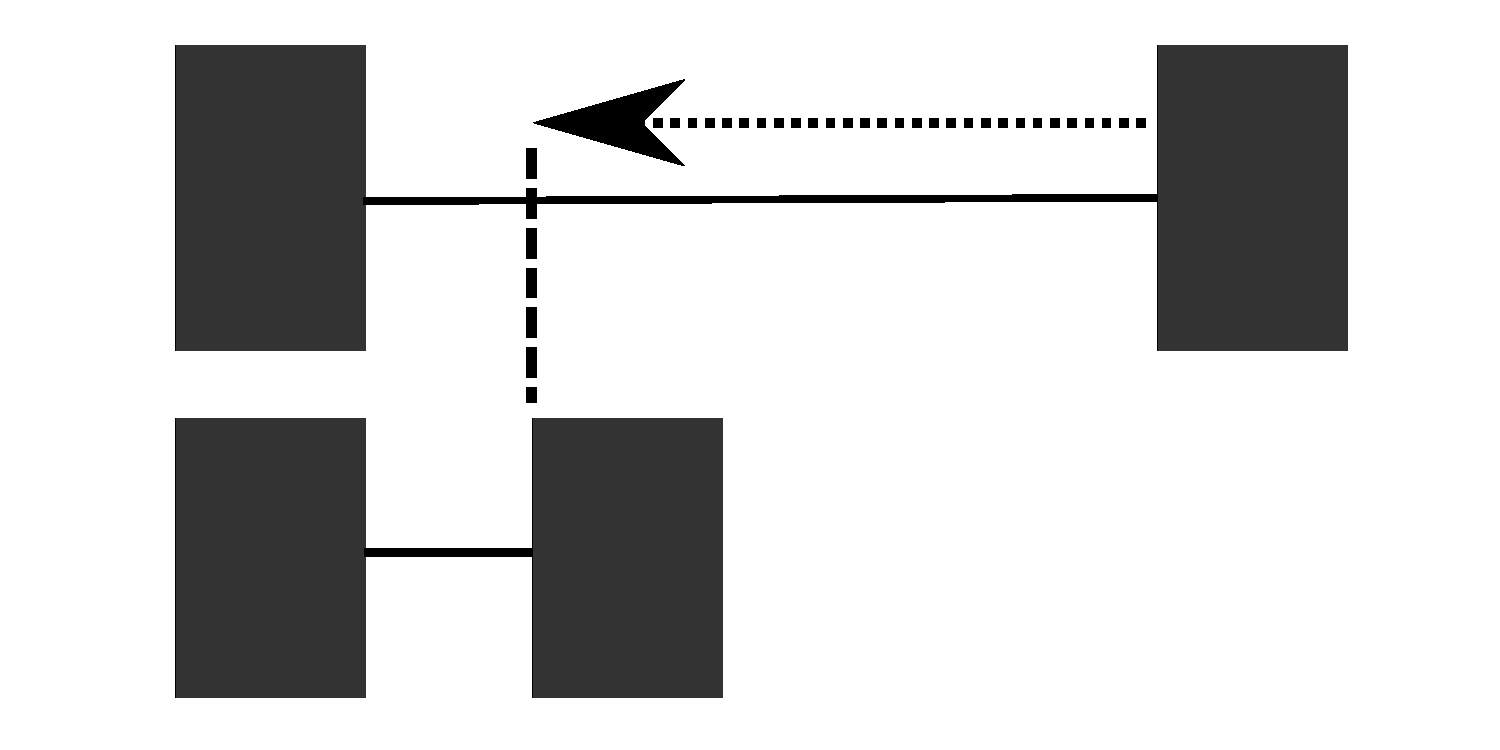
\includegraphics[height = 0.5cm]{figure/coord_truncate_gaps.pdf}\\\hline
\textbf{layout}&default & normal layout &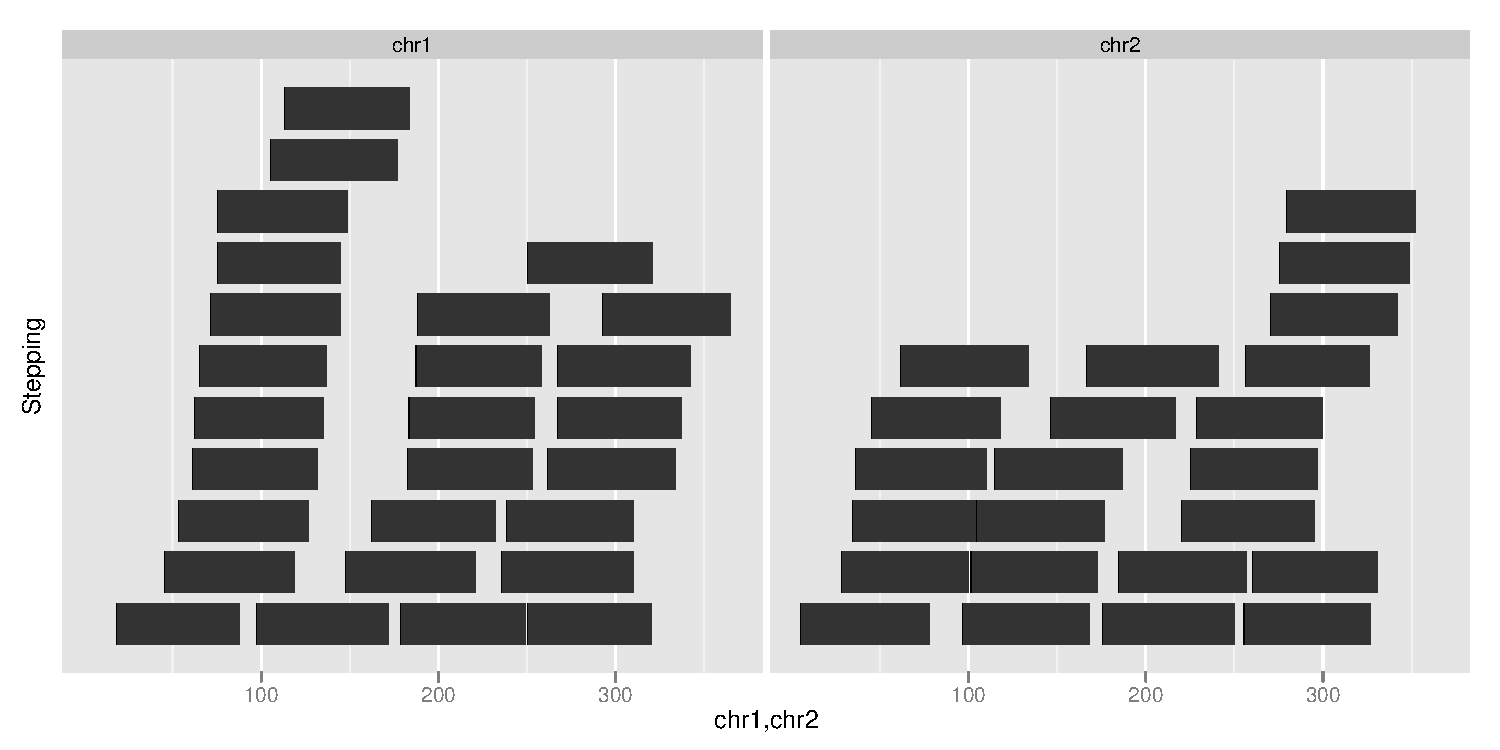
\includegraphics[height = 0.5cm]{figure/coord_linear.pdf}\\
              &karyogram & karyogram layout &
              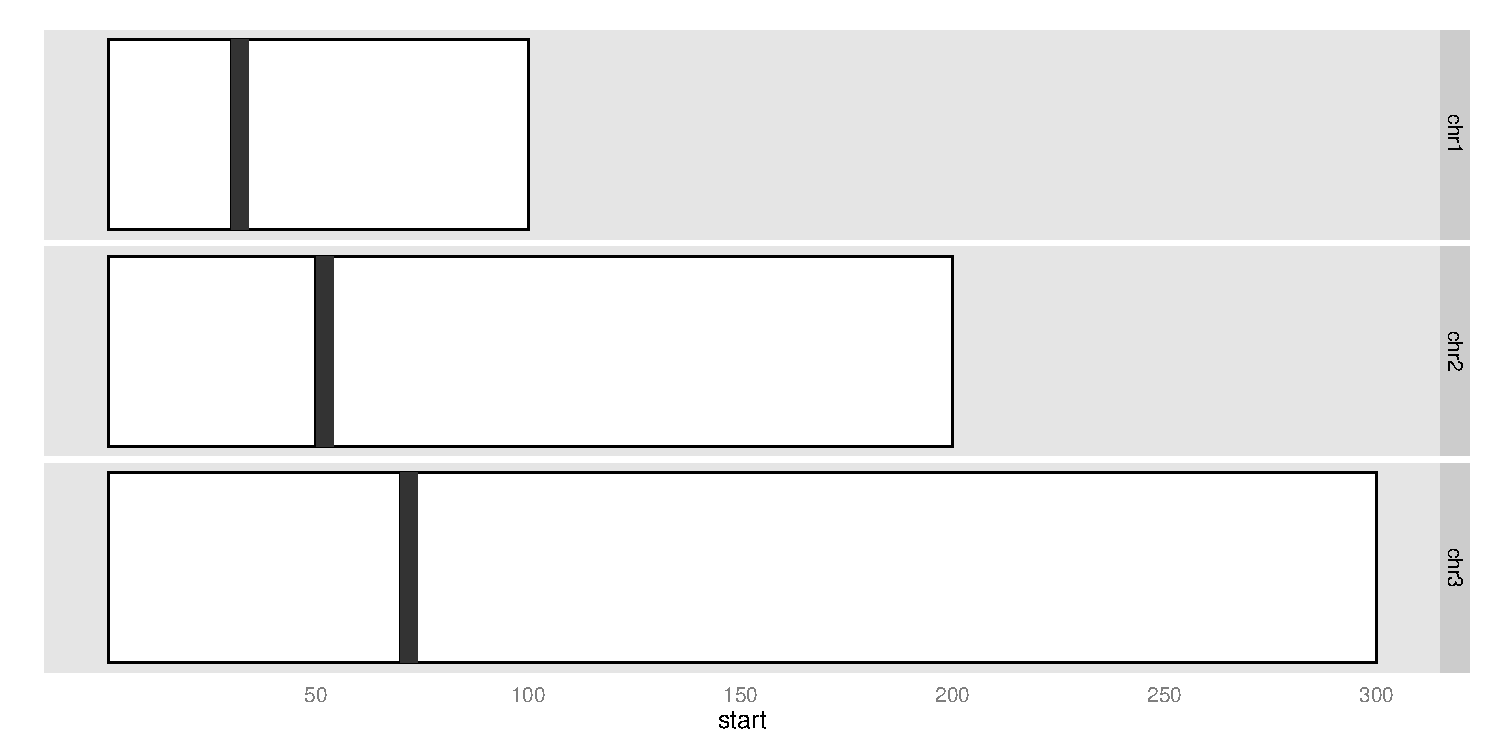
\includegraphics[height = 0.5cm]{figure/layout_karyogram.pdf}\\
              &circle & circular layout&
              
\includegraphics[height = 0.5cm]{figure/layout_circle.pdf}\\\hline
\textbf{faceting}&formula & formula based faceting&
               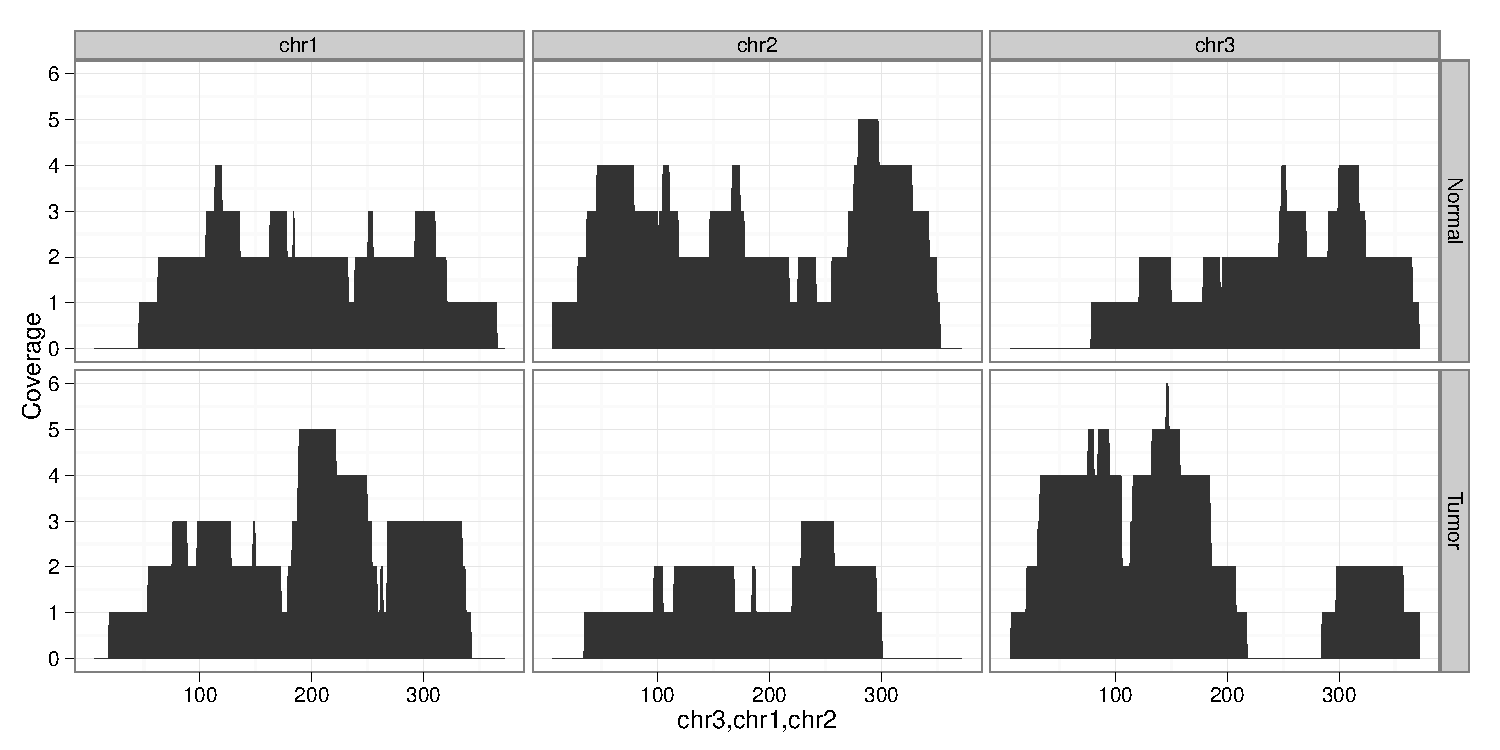
\includegraphics[height = 0.5cm]{figure/facet.pdf}\\
                 &ranges & ranges based faceting &
                 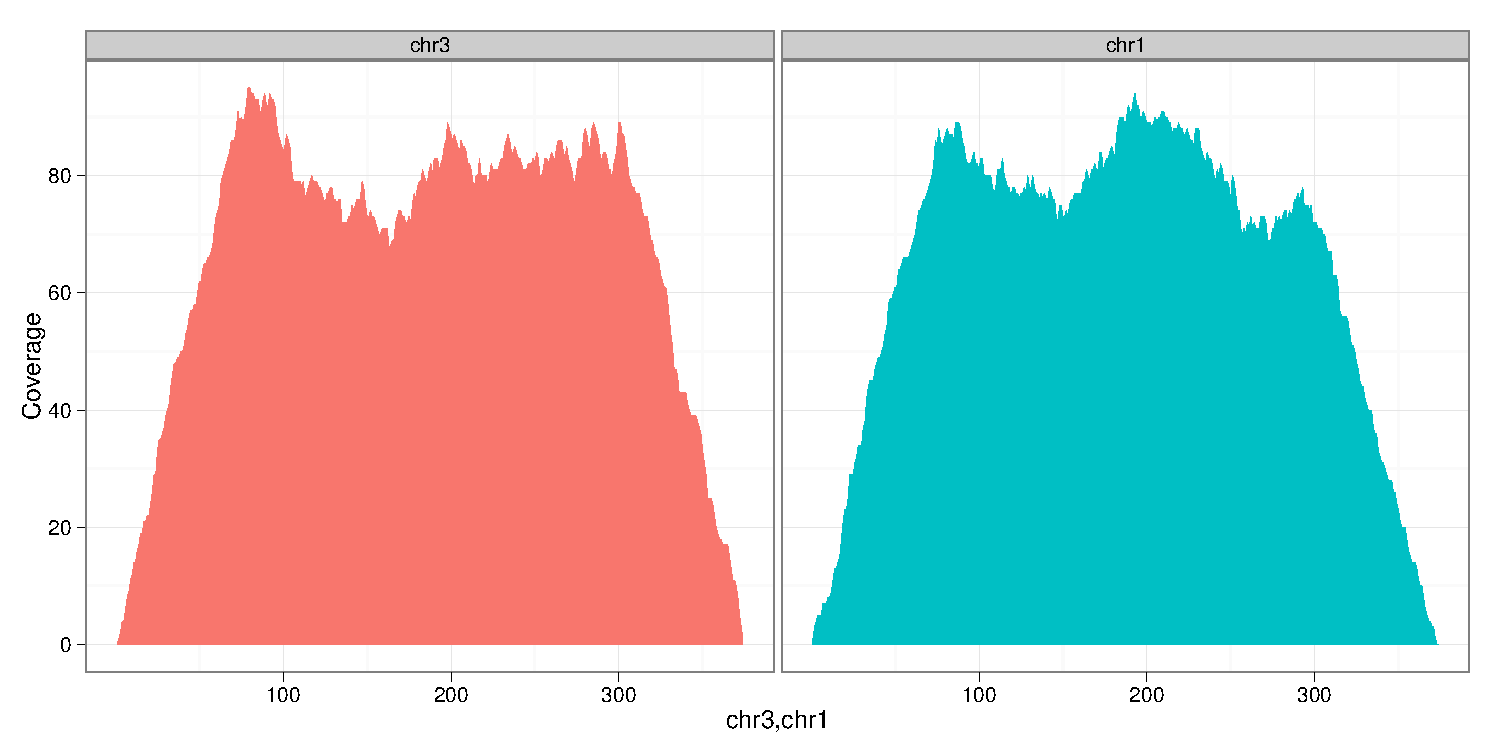
\includegraphics[height = 0.5cm]{figure/facet_gr.pdf}\\\hline
\textbf{scale} &not extended  & \ggplot{}default& \\\hline
\end{tabular}
}
\caption{Components of the basic grammar of graphics, with the extensions available in 
\ggbio{}.}
\label{tab:components}
\end{table}


\begin{table}[h!t!b!p]
\small{
\begin{tabular}{|p{4cm}|p{3cm}|p{2cm}|}
\hline
object & usage & icon\\\hline
GRanges & Genomic intervals&
\includegraphics[height = 0.5cm]{figure/geom_rect.pdf}\\\hline
GRangesList &Genomic interval list&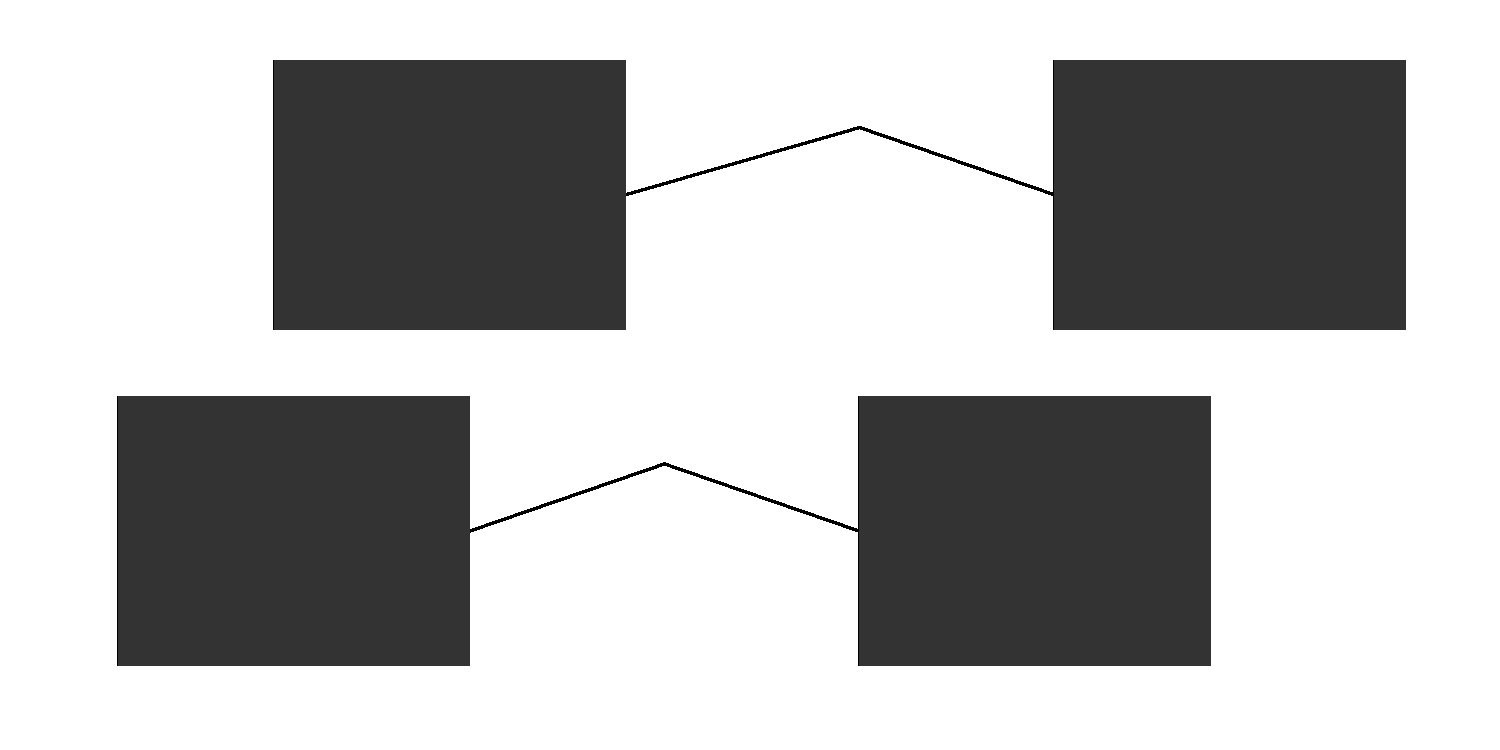
\includegraphics[height = 0.5cm]{figure/grl.pdf}\\\hline
IRanges&intervals&
\includegraphics[height = 0.5cm]{figure/stat_stepping.pdf}\\\hline
Gapped Alignments & gapped alignments&
 
\includegraphics[height = 0.5cm]{figure/stat_stepping.pdf}\\\hline
BamFile&alignemnts files&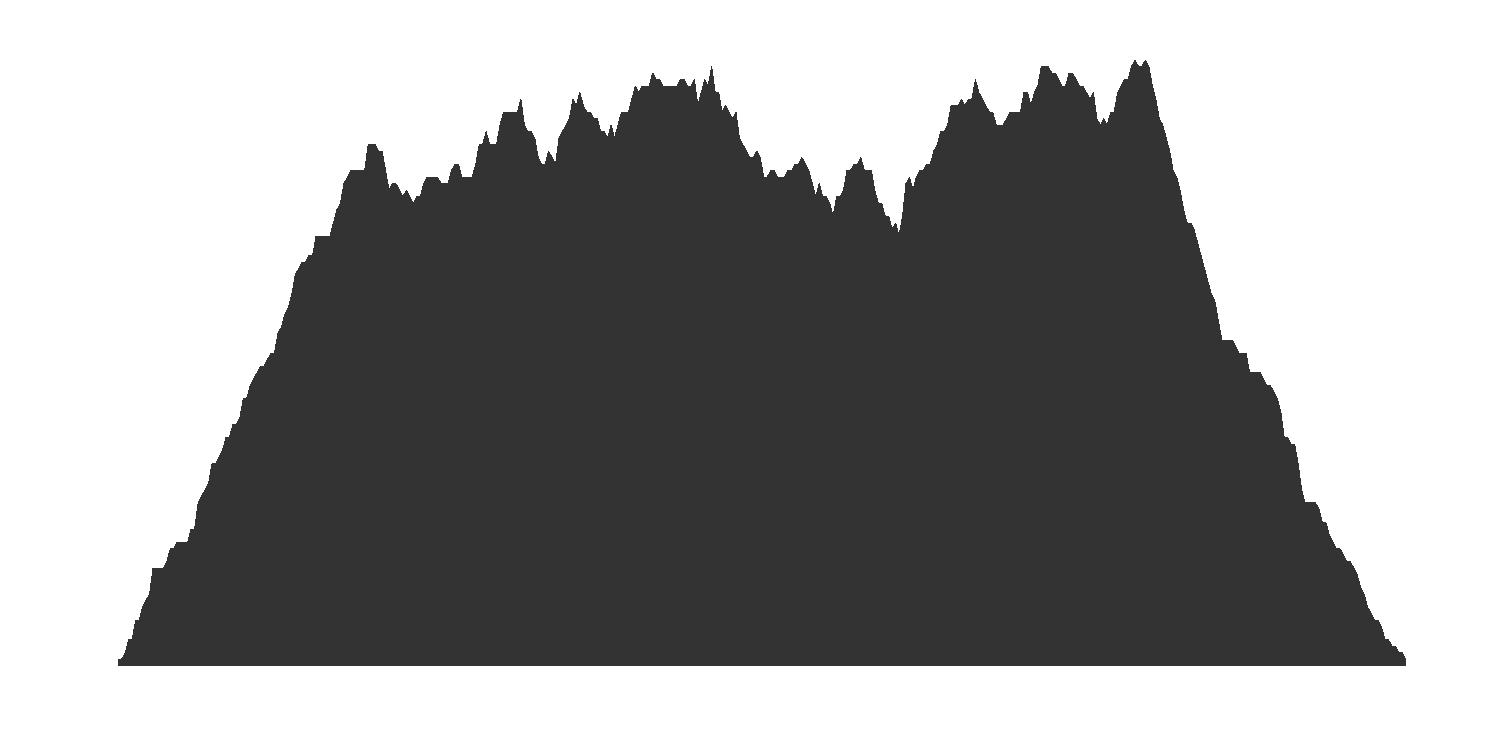
\includegraphics[height = 0.5cm]{figure/stat_coverage_icon.pdf}\\\hline
character&for flat files&
\includegraphics[height = 0.5cm]{figure/geom_bar.pdf}\\\hline
Rle/RleList&atomic vector&
\includegraphics[height = 0.5cm]{figure/stat_stepping.pdf}\\\hline
TranscriptDb&gene structure &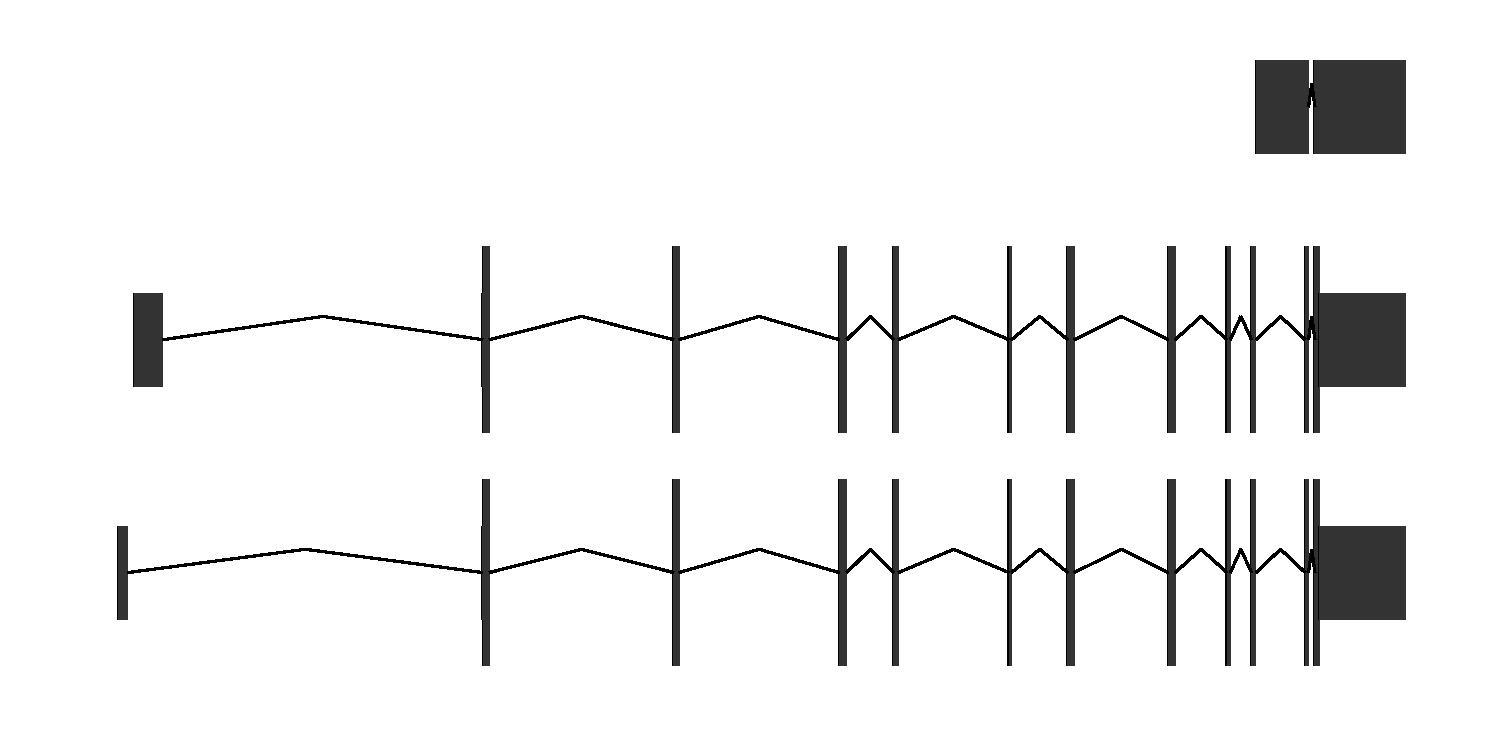
\includegraphics[height = 0.5cm]{figure/stat_gene.pdf}\\\hline
VCF&Variant calling format&
\includegraphics[height = 0.5cm]{figure/vcf.pdf}\\\hline
\end{tabular}
}
\caption{Formal data model and their default graphics}
\label{tab:model}
\end{table}

\end{document}
